\section{Specifications}
\newcounter{rulei}[subsection]
\newcommand{\rcnii}{\stepcounter{rulei}\arabic{section}.\arabic{subsection}.\arabic{rulei}}
\renewcommand{\labelenumi}{\rcnii}

\subsection{Arena}
\begin{enumerate}
\item The match arena is a 8m x 8m square.  The tolerance of the two arena dimensions is $\pm0.5m$.
\item The floor of the arena is made of white plastic coated hardboard.
\item The hardboard is joined with white Gaffer tape.
\item The arena walls are $600\pm100mm$ high and are made of the same material as the arena floor.
\item The wall-to-floor join is bridged in white Gaffer tape.
\end{enumerate}

\subsection{Tokens}
\label{tokens}

\begin {enumerate} 
\item Tokens are cubes of side 45$\pm5mm$.
\item Tokens weigh 40$\pm10g$
\end {enumerate}

\subsection{Zones}
\begin {enumerate}
\item The arena contains 4 zones.  Each zone is located at a corner of the arena.  See figure~\ref{fig:arena}.
\item A zone is a 1.5m x 1.5m square.  The tolerance of the zone dimensions is $\pm50mm$.
\item The zone is bounded by the zone border.  The zone border is $135\pm5mm$ (3 tokens) in width.
\item Each zone has an associated colour.  The zone border is this colour.
\item The zone is split into two areas.  The main zone and the bonus zone.  See figure~\ref{fig:zone}.
\item The bonus zone and main zone are divided by a piece of wood painted white, with a cross section that is the same size as a token - i.e. $45\pm5mm$.
\end {enumerate}

\begin{figure}
\begin{center}
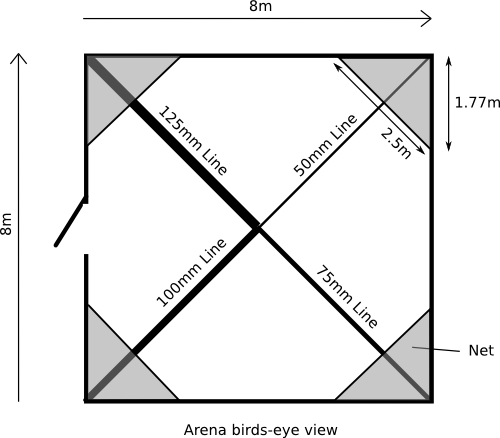
\includegraphics[keepaspectratio, width=\textwidth]{./images/arenadim.png}
\caption{\label{fig:arena}Zone Dimensions}
\end{center}
\end{figure}

\begin{figure}
\begin{center}
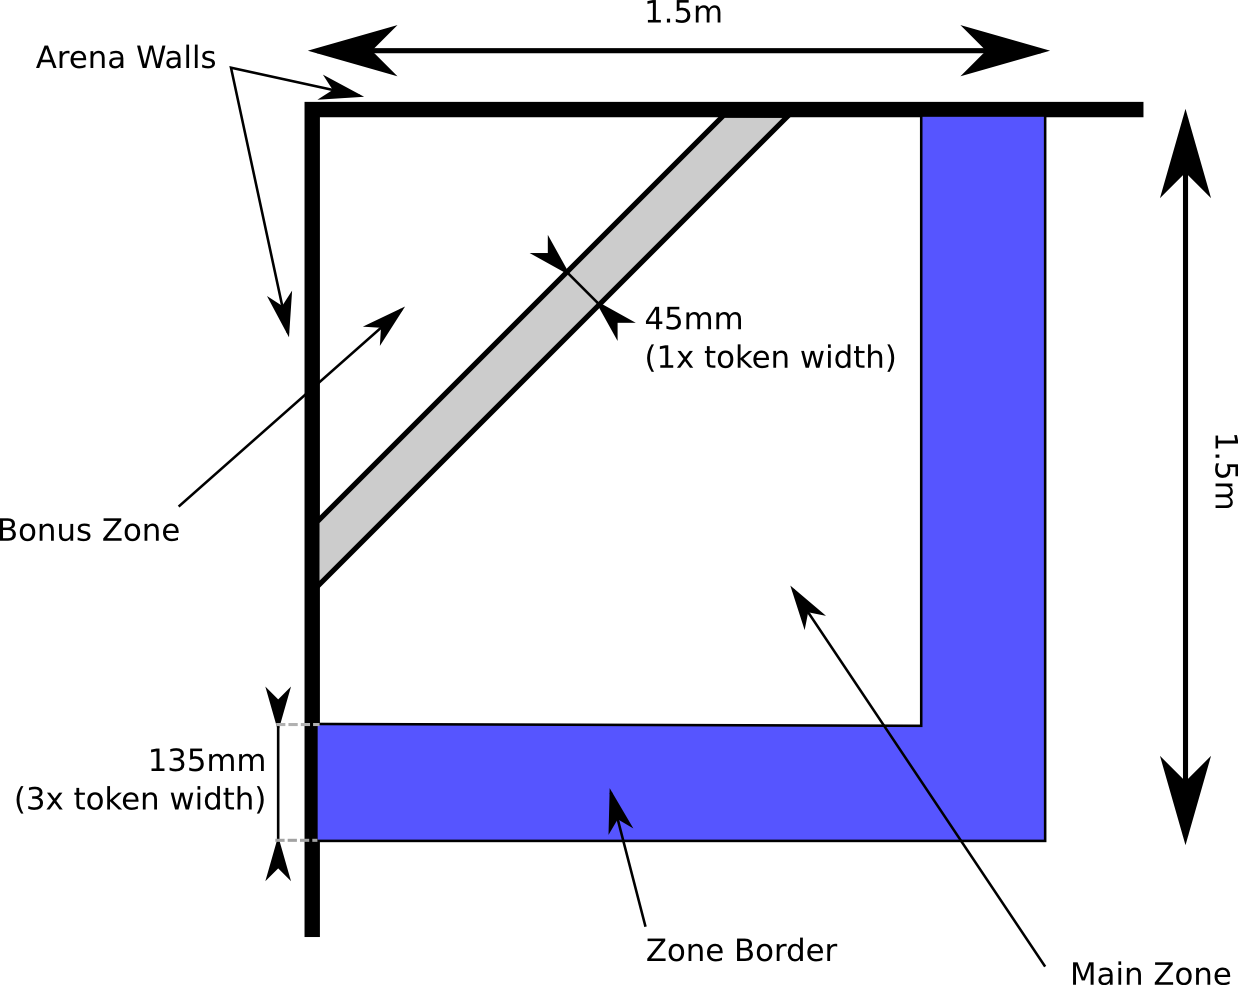
\includegraphics[keepaspectratio, scale =1]{./images/zone.png}
\caption{\label{fig:zone}Zone Dimensions}
\end{center}
\end{figure}

\subsection{Obstacles}
\begin{enumerate}
\item The arena will contain between 0 and 6 obstacles.
\item An obstacle is entirely black.
\item An obstacle has the shape described by figure~\ref{fig:obstacle}.
\end{enumerate}

\begin{figure}
\begin{center}
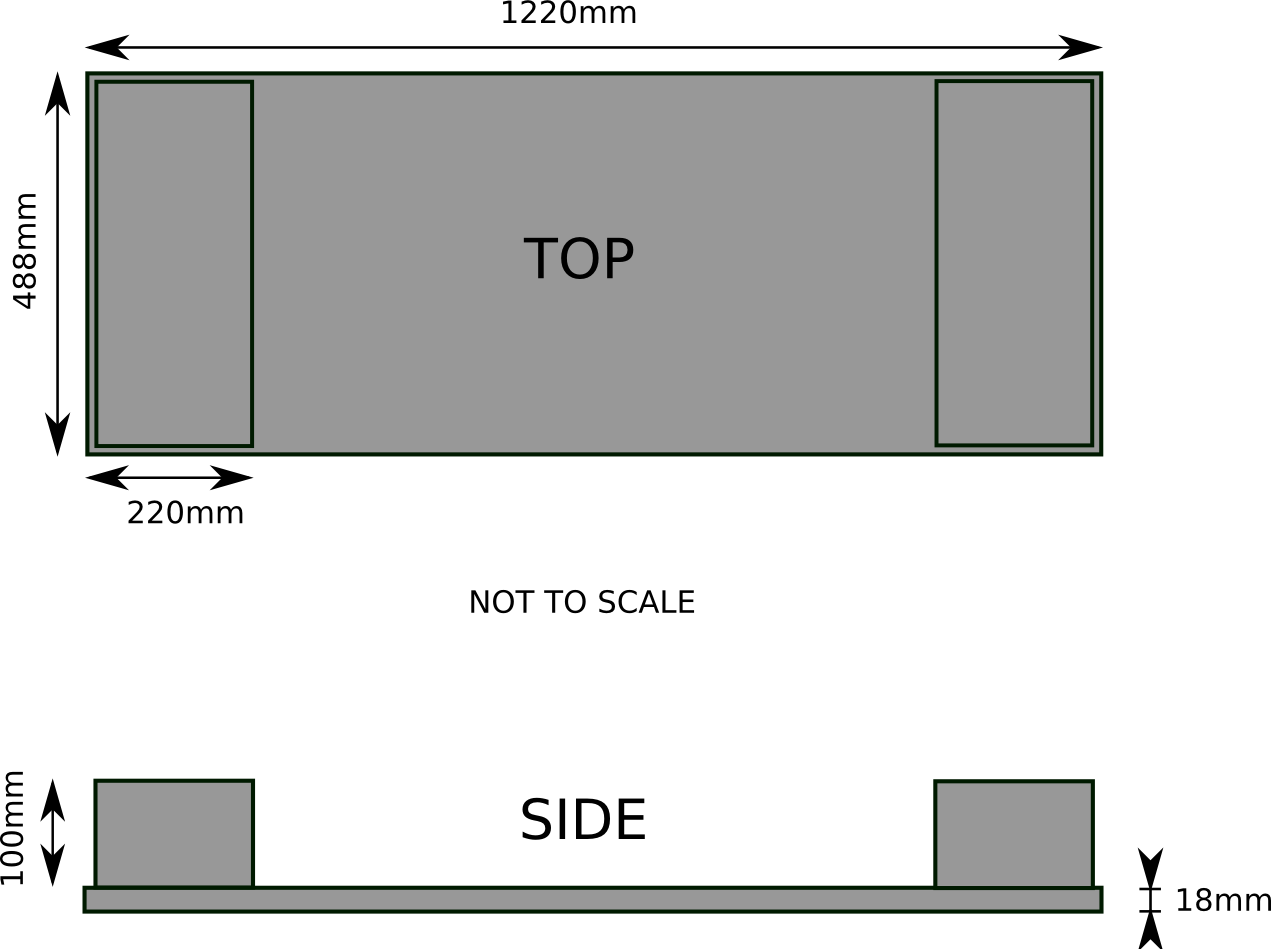
\includegraphics[keepaspectratio, scale =1]{./images/obstacle.png}
\caption{\label{fig:obstacle}Obstacle Dimensions}
\end{center}
\end{figure}
